% Complete RRT* → ground-speed MPC → ILOS → PWM control pipeline for a dual-thruster USV.
% Sensors assumed: GPS (position / velocity) + heading (+ optional gyro rate).
%   pdflatex mpc_ilos_pwm_pipeline.tex
\documentclass[11pt,a4paper]{article}

\usepackage[margin=2.2cm]{geometry}
\usepackage{lmodern}
\usepackage[T1]{fontenc}
\usepackage[utf8]{inputenc}
\usepackage{amsmath,amssymb,mathtools,bm}
\usepackage{booktabs}
\usepackage{enumitem}
\usepackage{xcolor}
\usepackage{listings}
\usepackage{tikz}
\usetikzlibrary{arrows.meta,positioning,fit,calc}
\usepackage[hidelinks]{hyperref}

\definecolor{accent}{HTML}{1F4E79}
\definecolor{soft}{HTML}{F4F7FB}
\definecolor{codebg}{HTML}{F7F7F7}

\lstset{
  basicstyle=\ttfamily\footnotesize,
  backgroundcolor=\color{codebg},
  frame=single,
  framerule=0.3pt,
  breaklines=true,
  columns=fullflexible,
  keepspaces=true
}

\setlist[itemize]{leftmargin=1.4em,itemsep=0.15em,topsep=0.25em}
\setlist[enumerate]{leftmargin=1.4em,itemsep=0.15em,topsep=0.25em}
\setlength{\parskip}{0.4em}
\setlength{\parindent}{0pt}

\title{\textbf{USV local control pipeline:\\
RRT$^\star$ waypoints $\rightarrow$ PWM}\\[0.35em]
\large Dual-thruster BlueBoat-class hull with
ground-speed kinematic MPC + ILOS}
\author{RefleXAI / LINC \quad---\quad mini\_bream notes}
\date{}

\begin{document}
\maketitle
\vspace{-1.2em}

\noindent
\textbf{Scope.}
Global path from RRT$^\star$; local \emph{ground-speed} MPC for short-horizon
obstacle avoidance; ILOS for path following under river current; cascade
surge/yaw control on GPS speed and heading; thruster allocation and map
\(f\) to PWM.
Custom sensor stack: \textbf{GPS + heading} (optional gyro).
No water-relative surge sensor (no DVL).
BlueBoat hull and thrusters only.

\begin{center}
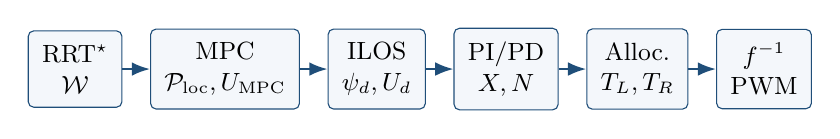
\begin{tikzpicture}[
  font=\small,
  box/.style={draw=accent, rounded corners=2pt, align=center,
              inner sep=5pt, fill=soft, minimum height=0.85cm},
  arr/.style={-{Latex}, accent, thick}
]
  \node[box] (w) {RRT$^\star$\\$\mathcal{W}$};
  \node[box, right=0.35cm of w] (m) {MPC\\$\mathcal{P}_{\mathrm{loc}},U_{\mathrm{MPC}}$};
  \node[box, right=0.35cm of m] (i) {ILOS\\$\psi_d,U_d$};
  \node[box, right=0.35cm of i] (c) {PI/PD\\$X,N$};
  \node[box, right=0.35cm of c] (a) {Alloc.\\$T_L,T_R$};
  \node[box, right=0.35cm of a] (f) {$f^{-1}$\\PWM};
  \draw[arr] (w) -- (m);
  \draw[arr] (m) -- (i);
  \draw[arr] (i) -- (c);
  \draw[arr] (c) -- (a);
  \draw[arr] (a) -- (f);
\end{tikzpicture}
\end{center}

%----------------------------------------------------------------------
\section{Notation and frames}
%----------------------------------------------------------------------

\begin{table}[h]
\centering
\small
\begin{tabular}{@{}ll@{}}
\toprule
Symbol & Meaning \\
\midrule
$\{n\}$ & Inertial frame (NED or ENU; fixed for the whole stack) \\
$\{b\}$ & Body frame: \(x\) forward, \(y\) starboard \\
$\eta=[x,y,\psi]^\top$ & Position and heading in \(\{n\}\) \\
$U_g$ & Speed over ground (m/s), from GPS \\
$\chi$ & Course over ground: \(\chi=\operatorname{atan2}(\dot y,\dot x)\) \\
$r$ & Yaw rate (rad/s), from gyro or \(\dot\psi\) \\
$U_k$ & MPC decision: commanded ground speed at step \(k\) \\
$B>0$ & Port--starboard thruster separation (m) \\
$T_L,T_R$ & Port / starboard thrust (N); forward \(>0\) \\
$n_L,n_R\in[-1,1]$ & Normalized thruster commands (or raw PWM \(\mu\)s) \\
$\Delta t_c$ & Inner-loop / ILOS period (e.g.\ \(0.02\,\mathrm{s}\)) \\
$\Delta t_m$ & MPC period (e.g.\ \(0.1\)--\(0.2\,\mathrm{s}\)) \\
\bottomrule
\end{tabular}
\end{table}

\textbf{Measurements.}
\(x,y\) from GNSS.
Prefer native GNSS velocity if available; otherwise
\[
\dot x \approx \frac{x_k-x_{k-1}}{\Delta t},\qquad
\dot y \approx \frac{y_k-y_{k-1}}{\Delta t}
\]
with light low-pass filtering, then
\[
U_g=\sqrt{\dot x^2+\dot y^2}.
\]
Heading \(\psi\) from AHRS/magnetometer; \(r\) from gyro if available.

\textbf{Design choice.}
The MPC and surge loop use \textbf{ground speed} only.
River current is rejected by ILOS integral action on cross-track error,
not by an explicit current state in the MPC.

%----------------------------------------------------------------------
\section{Global path (RRT$^\star$)}
%----------------------------------------------------------------------

\textbf{Output:} waypoint list
\[
\mathcal{W}=\{W_i\}_{i=0}^{N_w},\qquad
W_i=(x_i,y_i)\in\mathbb{R}^2,
\]
optionally with per-waypoint cruise ground speed \(U_i^{\mathrm{nom}}\).

\textbf{Active global segment:} \(W_i\to W_{i+1}\).
Advance \(i\) when \(\|p-W_{i+1}\|<R_{\mathrm{wp}}\) (e.g.\ \(1\)--\(2\,\mathrm{m}\)).

\textbf{Corridor for MPC:} densify/subsample the active segment (and a few ahead)
into a reference polyline \(\mathcal{P}_{\mathrm{ref}}\) in \(\{n\}\).

%----------------------------------------------------------------------
\section{Local ground-speed MPC (path generator)}
%----------------------------------------------------------------------

\textbf{Rate:} \(1/\Delta t_m\).
\textbf{Role:} short-horizon collision-free path near \(\mathcal{P}_{\mathrm{ref}}\);
does \emph{not} command thrusters.

\subsection{Decision variables (internal)}
Over horizon \(N\) steps with step \(\Delta t_m\):
\[
\{U_k,\, r_k\}_{k=0}^{N-1}
\quad\text{(ground-speed and yaw-rate commands).}
\]

\subsection{Prediction model}
\[
\begin{aligned}
x_{k+1}
  &= x_k + \Delta t_m\, U_k\cos\psi_k, \\
y_{k+1}
  &= y_k + \Delta t_m\, U_k\sin\psi_k, \\
\psi_{k+1}
  &= \psi_k + \Delta t_m\, r_k.
\end{aligned}
\]
Initial state: measured \((x,y,\psi)\).
No current term: prediction assumes motion at commanded ground speed along
heading; closed-loop GPS tracking of \(U_d\) and ILOS make this consistent
enough for a short horizon.

\subsection{Obstacles}
Track \(j\): center \(p_j\), velocity \(v_j\), radius \(R_j\).
Predict \(p_j(k)=p_j(0)+k\Delta t_m\,v_j\).
Safety radius:
\(R_{\mathrm{safe},j}=R_j+R_{\mathrm{boat}}+R_{\mathrm{margin}}\).

\subsection{Constraints}
\[
\begin{aligned}
0 \le U_{\min} &\le U_k \le U_{\max}, \\
|r_k| &\le r_{\max}, \\
|U_{k+1}-U_k| &\le \Delta U_{\max}, \\
|r_{k+1}-r_k| &\le \Delta r_{\max}, \\
\|(x_k,y_k)-p_j(k)\| &\ge R_{\mathrm{safe},j}
\quad\text{(hard, or soft with slack).}
\end{aligned}
\]
Motion limits are \emph{empirical GPS quantities}
(Section~\ref{sec:limits}), not water-relative surge limits.

\subsection{Cost (example)}
\[
J=\sum_{k=0}^{N}\Big(
w_p\, d^2\!\big((x_k,y_k),\mathcal{P}_{\mathrm{ref}}\big)
+ w_U(U_k-U_{\mathrm{nom}})^2
+ w_r r_k^2
+ w_{\Delta U}(\Delta U_k)^2
+ w_{\Delta r}(\Delta r_k)^2
\Big),
\]
where \(d(\cdot,\mathcal{P}_{\mathrm{ref}})\) is the shortest distance from the
point to the reference polyline (min distance to the clamped projection on
each segment).

\subsection{MPC outputs (interface to ILOS)}
After each solve, publish:

\begin{center}
\small
\begin{tabular}{@{}ll@{}}
\toprule
Output & Definition \\
\midrule
Local path \(\mathcal{P}_{\mathrm{loc}}=\{(x_k^*,y_k^*)\}_{k=0}^{N}\)
  & Predicted positions (polyline in \(\{n\}\)) \\
Speed ref \(U_{\mathrm{MPC}}:=U_0^*\)
  & First optimal ground speed (optional LPF / saturate) \\
\bottomrule
\end{tabular}
\end{center}

Do \emph{not} send \(\{r_k^*\}\) to ILOS.
On MPC fail/timeout: keep last \(\mathcal{P}_{\mathrm{loc}},U_{\mathrm{MPC}}\),
or fall back to \(W_i\to W_{i+1}\) with safe \(U_{\mathrm{nom}}\).

\noindent\textit{Note.}
\(U_k,r_k\) are optimizer variables used to generate \(\mathcal{P}_{\mathrm{loc}}\).
The published interface is the path and \(U_{\mathrm{MPC}}\), not open-loop \(r\).

%----------------------------------------------------------------------
\section{ILOS (path follower)}
%----------------------------------------------------------------------

\textbf{Rate:} \(1/\Delta t_c\) (or same as inner loops).\\
\textbf{Inputs:} \(\mathcal{P}_{\mathrm{loc}}\) (or global segment if no MPC path),
\(U_{\mathrm{MPC}}\), pose \((x,y,\psi)\).\\
\textbf{Outputs:} \(\psi_d,\, U_d\).

\subsection{Active local segment}
On \(\mathcal{P}_{\mathrm{loc}}\), take consecutive points \(A\to B\).
Let \(p=(x,y)\).
Cross-track error \(e\): signed distance from \(p\) to line \(AB\)
(fix a sign convention and keep it).
Advance when progress along \(AB\) exceeds segment length \(-\varepsilon\).

Path angle:
\[
\alpha=\operatorname{atan2}(y_B-y_A,\, x_B-x_A).
\]

\subsection{ILOS law}
Parameters: look-ahead \(\Delta>0\) (m), integral gain \(\sigma>0\) (m/s).
\[
\begin{aligned}
\dot e_I
  &= \frac{\Delta\, e}{\Delta^2+(e+\sigma e_I)^2}
  \quad\text{(Euler with \(\Delta t_c\); anti-windup if \(|e|\) large),} \\
\psi_d
  &= \alpha - \arctan\!\Big(\frac{e+\sigma e_I}{\Delta}\Big), \\
U_d
  &= \mathrm{sat}(U_{\mathrm{MPC}},\, U_{\min},U_{\max}).
\end{aligned}
\]

\textbf{River current / drift.}
Rejected by the integral state \(e_I\): under steady flow the boat crabs
(\(\psi_d\neq\alpha\)) while cross-track \(e\to 0\).
No current estimate is required in ILOS or in the MPC.

Unwrap \(\psi_d-\psi\) to \((-\pi,\pi]\) in the yaw controller.

%----------------------------------------------------------------------
\section{Inner controllers $\rightarrow$ body force / moment}
%----------------------------------------------------------------------

\textbf{Inputs:} \(U_d,\psi_d\); measured \(U_g,\psi,r\).\\
\textbf{Outputs:} surge force \(X\) (N), yaw moment \(N\) (N$\cdot$m).

\subsection{Surge (PI) on ground speed}
\[
X = K_{p,U}(U_d-U_g) + K_{i,U}\int(U_d-U_g)\,dt,
\]
with \(X\in[X_{\min},X_{\max}]\) and integrator anti-windup.
Optional: use longitudinal ground speed
\(U_g\cos(\chi-\psi)\) instead of \(U_g\) if crab is large.

\subsection{Yaw (PD on heading)}
\[
N = K_{p,\psi}\,e_\psi - K_{d,\psi}\, r,\qquad
e_\psi=\operatorname{wrap}(\psi_d-\psi),
\]
with \(N\in[-N_{\max},N_{\max}]\).

Cascade alternative: \(r_d=K_\psi e_\psi\), then \(N=K_r(r_d-r)\).

\(X\) and \(N\) are \emph{computed} by these controllers; they are not measured.

%----------------------------------------------------------------------
\section{Control allocation}
%----------------------------------------------------------------------

\textbf{Inputs:} \(X,N\).
\textbf{Outputs:} \(T_L,T_R\).

Ideal dual-thruster map (no lateral actuator):
\[
X=T_L+T_R,\qquad
N=\frac{B}{2}(T_L-T_R).
\]
Inversion:
\begin{equation}
\boxed{
T_L=\frac{X}{2}+\frac{N}{B},\qquad
T_R=\frac{X}{2}-\frac{N}{B}.
}
\end{equation}
Then saturate \(T_L,T_R\in[T_{\min},T_{\max}]\).
If both limits bind, re-scale (simple: clip; better: prioritize \(N\) near obstacles).

%----------------------------------------------------------------------
\section{Thruster map $f$: thrust $\leftrightarrow$ command}
%----------------------------------------------------------------------

\textbf{Definition.}
\[
T=f(n),\qquad
n=f^{-1}(T),
\]
with \(n\in[-1,1]\) (or PWM \(\mu\)s).
Actuate \(n_L=f^{-1}(T_L)\), \(n_R=f^{-1}(T_R)\).

\textbf{Typical grey-box shape} (deadband \(n_{\mathrm{db}}\); separate fwd/rev):
\[
f(n)=\begin{cases}
c_1^+ n + c_2^+ n|n|, & n\ge n_{\mathrm{db}}, \\
0, & |n|<n_{\mathrm{db}}, \\
c_1^- n + c_2^- n|n|, & n\le -n_{\mathrm{db}}.
\end{cases}
\]
Alternatively: manufacturer force-vs-PWM table (e.g.\ T200) with interpolation.

%----------------------------------------------------------------------
\section{Identifying $f$ and $B$ on a new boat}
\label{sec:sysid}
%----------------------------------------------------------------------

\begin{enumerate}
  \item \textbf{Measure \(B\):} distance between thruster axes (m).
  \item \textbf{Static map \(f\):}
    bollard/load-cell sweep of \(n\in[-1,1]\), or datasheet PWM$\to$force
    (rescale if ducting differs). Fit \(c_1^\pm,c_2^\pm,n_{\mathrm{db}}\)
    or store a lookup and its inverse.
  \item \textbf{Force limits:}
    \(T_{\min}=\min f\), \(T_{\max}=\max f\) (or \(\sim 0.9\) of peak).
    \(X_{\max}=2T_{\max}\),
    \(N_{\max}=(B/2)(T_{\max}-T_{\min})\) at extreme differential thrust.
  \item \textbf{Validate \(f^{-1}\):} command known \(T\); check surge/yaw response on GPS.
\end{enumerate}
Tune ILOS \((\Delta,\sigma)\) and PID gains after \(f\) exists (calm water, then river).
MPC motion limits are obtained separately by the field procedure below.

%----------------------------------------------------------------------
\section{Field procedure: MPC ground-speed limits}
\label{sec:limits}
%----------------------------------------------------------------------

Limits \(U_{\max}\), \(r_{\max}\), \(\Delta U_{\max}\), \(\Delta r_{\max}\) are
measured with GPS (+ heading/gyro). Prefer conservative values
(\(\sim 80\)--\(90\%\) of peaks) so closed-loop tracking can follow the plan.

\subsection{Quantities}
\begin{center}
\small
\begin{tabular}{@{}ll@{}}
\toprule
Symbol & Meaning \\
\midrule
$U_{\min},U_{\max}$ & Ground-speed command bounds \\
$r_{\max}$ & Max yaw rate \\
$\Delta U_{\max}$ & Max \(\lvert U_{k+1}-U_k\rvert\) per MPC step \(\Delta t_m\) \\
$\Delta r_{\max}$ & Max \(\lvert r_{k+1}-r_k\rvert\) per MPC step \\
$R_{\mathrm{margin}}$ & Extra obstacle inflation (m) \\
\bottomrule
\end{tabular}
\end{center}

\subsection{Tests}
\begin{enumerate}
  \item \textbf{\(U_{\max}\) --- straight surge runs.}
    Equal thrusters at several levels (e.g.\ 40\%, 60\%, 80\%, 100\%).
    Hold until \(U_g\) settles (\(10\)--\(30\,\mathrm{s}\)).
    Set \(U_{\max}\approx 0.85\)--\(0.9\times U_g^{\mathrm{peak}}\).
    In a river, repeat \emph{upstream and downstream}; use
    \(U_{\max}=\min(U_g^{\mathrm{up}},U_g^{\mathrm{down}})\) for a single
    conservative limit, or schedule by heading vs channel direction.
    Set \(U_{\min}=0\) or a small crawl (e.g.\ \(0.1\,\mathrm{m/s}\)).

  \item \textbf{\(r_{\max}\) --- spins / hard turns.}
    Max differential thrust CW and CCW, from rest and from cruise.
    Record peak \(\lvert r\rvert\) (gyro) or \(\lvert\dot\psi\rvert\).
    Set \(r_{\max}\approx 0.8\times\lvert r\rvert_{\mathrm{peak}}\).

  \item \textbf{\(\Delta U_{\max}\), \(\Delta r_{\max}\) --- accel limits.}
    Step thrust from rest (or from a steady speed); log filtered \(U_g(t)\).
    \[
      a_{\max}\approx\max\lvert\dot U_g\rvert
      \quad\Rightarrow\quad
      \Delta U_{\max}=a_{\max}\,\Delta t_m.
    \]
    Step differential thrust; likewise
    \(\Delta r_{\max}=\alpha_{\max}\,\Delta t_m\) with
    \(\alpha_{\max}\approx\max\lvert\dot r\rvert\).
    If derivatives are noisy, use a ramp fit over \(0.5\)--\(1\,\mathrm{s}\).

  \item \textbf{Closed-loop check.}
    With surge/yaw PIDs running, command steps in \(U_d\) and \(\psi_d\).
    If thrusters saturate before the command is reached, \emph{lower}
    the MPC limits. Limits must be what closed-loop tracking can hold.

  \item \textbf{\(R_{\mathrm{margin}}\).}
    Start with
    \(R_{\mathrm{margin}}\gtrsim U_{\max}\,t_{\mathrm{lag}}+\text{GPS noise}
    +\text{tracking error}\)
    (often \(0.5\)--\(1.5\,\mathrm{m}\) on a small boat); tighten with data.
\end{enumerate}

\subsection{Minimal half-day card}
\begin{enumerate}
  \item Three straight runs (slow / mid / max) \(\Rightarrow U_{\max}\).
  \item Upstream and downstream repeats in river \(\Rightarrow\) maybe reduce \(U_{\max}\).
  \item Four max yaw spins (CW/CCW \(\times 2\)) \(\Rightarrow r_{\max}\).
  \item One surge step + one yaw step \(\Rightarrow \Delta U_{\max},\Delta r_{\max}\).
  \item Optional closed-loop square/zigzag at those limits; trim \(10\)--\(20\%\) if lagging.
\end{enumerate}

%----------------------------------------------------------------------
\section{End-to-end online loops}
%----------------------------------------------------------------------

\begin{lstlisting}
offline:
  measure B; identify f, f^{-1}
  field-test U_max, r_max, dU_max, dr_max (GPS)
  set T/X/N limits; tune PIDs & ILOS

online @ Delta t_m  (MPC):
  read eta, U_g, r, obstacle tracks, P_ref from W
  solve ground-speed kinematic MPC
  publish P_loc, U_MPC

online @ Delta t_c  (ILOS + control):
  read eta, U_g, r, latest P_loc, U_MPC
  ILOS  ->  psi_d, U_d
  surge PI on (U_d - U_g)  ->  X
  yaw PD                   ->  N
  allocate  ->  T_L, T_R  (clip)
  n_L = f^{-1}(T_L),  n_R = f^{-1}(T_R)
  write PWM / ESC commands
\end{lstlisting}

%----------------------------------------------------------------------
\section{Signal dictionary}
%----------------------------------------------------------------------

\begin{table}[h]
\centering
\small
\begin{tabular}{@{}llll@{}}
\toprule
Name & Type & Produced by & Consumed by \\
\midrule
$\mathcal{W}$ & waypoint list & RRT$^\star$ & segment / $\mathcal{P}_{\mathrm{ref}}$ \\
$\mathcal{P}_{\mathrm{ref}}$ & polyline & global slicer & MPC cost \\
obstacles & $p_j,v_j,R_j$ & perception & MPC constraints \\
$U_g$ & scalar & GPS velocity & surge PI, monitoring \\
$\mathcal{P}_{\mathrm{loc}}$ & polyline & MPC & ILOS \\
$U_{\mathrm{MPC}}$ & scalar & MPC & ILOS $\to U_d$ \\
$\psi_d,U_d$ & scalars & ILOS & inner loops \\
$X,N$ & force, moment & PI / PD & allocation \\
$T_L,T_R$ & thrusts & allocation & $f^{-1}$ \\
$n_L,n_R$ & commands & $f^{-1}$ & ESCs \\
\bottomrule
\end{tabular}
\end{table}

\vspace{0.5em}
\noindent
\textbf{One-line summary.}
RRT$^\star$ gives global waypoints;
ground-speed MPC redraws a short collision-free polyline and a GPS speed hint;
ILOS tracks that polyline under current via \(e_I\) and passes \(U_d\);
PI/PD on \((U_d-U_g)\) and heading produce \(X,N\);
allocation and \(f^{-1}\) produce thruster PWM.

\end{document}
